% arXiv builds with pdflatex, where \pdfoutput=1 selects PDF output.
% The guard keeps local XeTeX-based builds working.
\ifdefined\XeTeXversion\else\ifdefined\pdfoutput\pdfoutput=1\fi\fi
\documentclass[10pt,twocolumn]{article}

\usepackage[letterpaper,top=0.80in,bottom=0.90in,left=0.68in,right=0.68in,columnsep=0.25in]{geometry}
\usepackage{amsmath,amssymb,amsthm,mathtools}
\usepackage{booktabs}
\usepackage{array}
\usepackage{graphicx}
\usepackage{microtype}
\usepackage{xcolor}
\usepackage{enumitem}
\usepackage{caption}
\usepackage{tikz}
\usepackage{pgfplots}
\usepackage{fancyhdr}
\usepackage[hidelinks]{hyperref}

\pgfplotsset{compat=1.16}

\definecolor{linkblue}{RGB}{20,65,125}
\definecolor{chartgray}{RGB}{94,94,94}
\definecolor{chartlight}{RGB}{158,158,158}
\hypersetup{
  colorlinks=true,
  linkcolor=linkblue,
  citecolor=linkblue,
  urlcolor=linkblue,
  pdfauthor={Mehmet Demir Guven},
  pdftitle={Spurious or Structural? Low-Rank Confounding and Partial Identification of Cross-Asset Price Impact},
  pdfsubject={Preprint and pre-results research protocol},
  pdfkeywords={cross-impact, order-flow imbalance, latent factors, partial identification, preregistration}
}

% ---- page furniture: preprint mark on every page, including the first -------
\pagestyle{fancy}
\fancyhf{}
\fancyfoot[C]{\small Preprint. Under review.}
\fancyfoot[R]{\small\thepage}
\renewcommand{\headrulewidth}{0pt}
\renewcommand{\footrulewidth}{0.4pt}
\fancypagestyle{plain}{%
  \fancyhf{}%
  \fancyfoot[C]{\small Preprint. Under review.}%
  \fancyfoot[R]{\small\thepage}%
  \renewcommand{\headrulewidth}{0pt}%
  \renewcommand{\footrulewidth}{0.4pt}%
}

\newcommand\daggerfootnote[1]{%
  \begingroup
  \renewcommand\thefootnote{}\footnote{#1}%
  \addtocounter{footnote}{-1}%
  \endgroup
}

\setlength{\parindent}{1em}
\setlength{\parskip}{0pt}
\setlist[itemize]{leftmargin=1.25em,itemsep=2pt,topsep=3pt}
\setlist[enumerate]{leftmargin=1.35em,itemsep=2pt,topsep=3pt}
\captionsetup{font=small,labelfont=bf}

\newtheorem{theorem}{Theorem}
\newtheorem{proposition}{Proposition}
\newtheorem{corollary}{Corollary}
\newtheorem{definition}{Definition}
\theoremstyle{remark}
\newtheorem{remark}{Remark}

\newcommand{\R}{\mathbb{R}}
\newcommand{\E}{\operatorname{E}}
\newcommand{\Var}{\operatorname{Var}}
\newcommand{\Cov}{\operatorname{Cov}}
\newcommand{\plim}{\operatorname{plim}}
\newcommand{\tr}{\operatorname{tr}}
\newcommand{\rank}{\operatorname{rank}}
\newcommand{\col}{\operatorname{col}}
\newcommand{\sym}{\operatorname{sym}}
\newcommand{\spann}{\operatorname{span}}
\newcommand{\diag}{\operatorname{diag}}

% Generated by python -m xid.exhibits. Do not edit by hand.
\newcommand{\FigBoundsUpper}{(0.1,0.09627798096) (0.1125,0.09784909501) (0.125,0.09897860681) (0.1375,0.09981426819) (0.15,0.1004465555) (0.1625,0.100933689) (0.175,0.1013146525) (0.1875,0.1016164168) (0.2,0.1018581609) (0.2125,0.1020538463) (0.225,0.1022138454) (0.2375,0.1023460036) (0.25,0.1024563504) (0.2625,0.1025495882) (0.275,0.1026294334) (0.2875,0.1026988611) (0.3,0.1027602816) (0.3125,0.1028156714) (0.325,0.1028666702) (0.3375,0.1029146551) (0.35,0.1029607974) (0.3625,0.1030061063) (0.375,0.1030514639) (0.3875,0.1030976526) (0.4,0.1031453773) (0.4125,0.1031952837) (0.425,0.1032479737) (0.4375,0.1033040182) (0.45,0.1033639679)}
\newcommand{\FigBoundsLower}{(0.1,-0.06470302689) (0.1125,-0.06697572531) (0.125,-0.06878903937) (0.1375,-0.07027340085) (0.15,-0.07151370079) (0.1625,-0.07256777024) (0.175,-0.07347646952) (0.1875,-0.07426954586) (0.2,-0.07496920652) (0.2125,-0.0755923891) (0.225,-0.07615225408) (0.2375,-0.07665919529) (0.25,-0.07712154158) (0.2625,-0.07754605478) (0.275,-0.07793829036) (0.2875,-0.07830286302) (0.3,-0.0786436456) (0.3125,-0.07896392002) (0.325,-0.0792664935) (0.3375,-0.07955378905) (0.35,-0.07982791683) (0.3625,-0.08009073099) (0.375,-0.08034387548) (0.3875,-0.08058882138) (0.4,-0.0808268976) (0.4125,-0.08105931653) (0.425,-0.08128719561) (0.4375,-0.08151157585) (0.45,-0.08173343786)}
\newcommand{\FigBoundsObserved}{(0.1,0.01578747703) (0.1125,0.01543668485) (0.125,0.01509478372) (0.1375,0.01477043367) (0.15,0.01446642734) (0.1625,0.01418295938) (0.175,0.01391909149) (0.1875,0.01367343548) (0.2,0.01344447718) (0.2125,0.01323072858) (0.225,0.01303079566) (0.2375,0.01284340413) (0.25,0.01266740442) (0.2625,0.01250176669) (0.275,0.01234557152) (0.2875,0.01219799903) (0.3,0.01205831802) (0.3125,0.01192587569) (0.325,0.01180008833) (0.3375,0.01168043301) (0.35,0.01156644026) (0.3625,0.01145768765) (0.375,0.01135379422) (0.3875,0.01125441561) (0.4,0.01115923982) (0.4125,0.01106798358) (0.425,0.01098038907) (0.4375,0.01089622117) (0.45,0.01081526502)}

% Generated by python -m xid.exhibits. Do not edit by hand.
\newcommand{\FigPsiCurve}{(0,0) (0.01,0.003915312523) (0.02,0.007830023456) (0.05,0.01956826134) (0.1,0.03909868631) (0.15,0.05856304262) (0.2,0.07793358954) (0.3,0.1162858754)}
\newcommand{\FigPsiByFactorCount}{(1,0.6396312102) (2,0.3748434626) (3,0.03909868631) (4,0.03766612117) (6,0.03276644296) (10,0.02498804432)}

% Generated by python -m xid.exhibits from the committed psi study.
\newcommand{\FigPsiSize}{(500,0.2666666667) (1000,0.1266666667) (2000,0.1) (5000,0.04)}
\newcommand{\FigPsiPower}{(0.05,0.07) (0.1,0.27) (0.2,0.87) (0.4,1)}


\begin{document}

\twocolumn[
\begin{@twocolumnfalse}
\begin{center}
\rule{\textwidth}{1.1pt}\vspace{5pt}

{\LARGE\bfseries Spurious or Structural?\\[4pt]
Low-Rank Confounding and Partial Identification\\
of Cross-Asset Price Impact\par}

\vspace{7pt}
\rule{\textwidth}{0.5pt}

\vspace{9pt}
{\large Mehmet Demir G\"uven\textsuperscript{\dag}\par}
\vspace{4pt}
{\normalsize\bfseries ETH Z\"urich\par}
\vspace{3pt}
{\small \texttt{dgueven@student.ethz.ch}\par}
\end{center}

\vspace{13pt}
\begin{center}
\begin{minipage}{0.895\textwidth}
\centerline{\textsc{Abstract}}
\vspace{4pt}
\normalsize
Cross-asset return-on-flow coefficients are routinely read as entries of a
structural price-impact matrix. That reading is generically unidentified. We
treat cross-impact as an identification problem and carry it through four
stages: what fails, what survives, what can be refuted, and what would restore
it. In a simultaneous $N$-asset system with $K$ latent factors and same-bin
feedback $B$, the gap between the population regression coefficient and the
structural matrix has rank at most $K+\rank(B)$, and we prove the bound is
attained --- exactly, away from an explicit exceptional set, with the corollary
that the theory has no testable content once $K+\rank(B)$ reaches $N$. A
strictly diagonal truth induces spurious cross terms of $0.221$ against own
terms spanning $0.206$ to $0.395$, and at published one-minute commonality
statistics the sharp identified interval for the off-diagonal runs from
$-0.078$ to $0.103$ around an observed $0.012$: not identified even in sign.
What survives is characterised completely. With
$W=\Sigma_{qq}^{-1}\Delta_f$, the functional $a^\top\Lambda b$ is point
identified if and only if $W^\top b=0$ and the cost $x^\top\Lambda x$ if and
only if $W^\top x=0$ --- a condition on the trade, not on the matrix, and one
that binds the flow argument alone. Parameter identification and decision
identification are different objects, and the second is more forgiving than the
first: a trader optimising against the confounded matrix under a linear
constraint suffers regret that is exactly the true cost of the trade error and
is \emph{second order} in the confounding, $0.015\%$ of optimal cost at a gap
that leaves entries badly wrong. The pure-confounding null is refutable without
estimating any nuisance: disjoint cross-blocks of the coefficient matrix
satisfy $\rank(A_{I,J})\le K$ exactly, giving tetrad restrictions on four
observed entries at $K=1$ and a certified lower bound on the minimum
confounding dimension $K_{\min}(A)$, whose comparison with an independently
estimated flow-factor count is the sharp empirical test. Finally, identification
is restorable: one noisy factor proxy does not identify $\Lambda$, but two
conditionally independent proxies point identify it in closed form. We verify
the theory in a preregistered known-truth experiment with $N=30$, $K=3$,
$T=10^{7}$, and register, without reporting, a falsification protocol for the
empirical stage.
\end{minipage}
\end{center}

\vspace{12pt}
\end{@twocolumnfalse}
]

\thispagestyle{fancy}

\daggerfootnote{\textsuperscript{\dag}\,Independent research. ETH Z\"urich did
not fund, sponsor, approve, or endorse this work. The affiliation records the
author's status as a student only, and the views expressed are the author's
alone. Correspondence: \texttt{dgueven@student.ethz.ch}.}

\section{Introduction}

Consider a fact from the published cross-impact literature. Capponi and Cont
\cite{CapponiCont2020} regress one-minute returns on the order-flow imbalance
of every stock in a large cross-section and report a mean cross-asset
coefficient of $+0.032$, with $23.09\%$ of those coefficients negative. They
then add a single cross-sectional principal-component control. The mean cross
coefficient becomes $-0.039$ and the negative share rises to $84.46\%$.

One control flips the sign of the average estimated cross-impact. Two readings
are available. Either the uncontrolled regression was contaminated and the
controlled one reveals the true structural effect, or the control absorbed real
impact and the uncontrolled one was right. The literature has no decisive way
to choose, and the choice matters: structural impact matrices enter
execution-cost models, liquidity stress tests, and manipulation constraints,
where a sign error is not a rounding error.

This paper argues that neither reading is identified, and makes that claim
precise rather than rhetorical.

Our starting point is the standard simultaneous system in which returns load on
flows, flows load on returns within the same bin, and both load on latent
common factors. The population coefficient of a return-on-flow regression
equals the structural impact matrix plus a discrepancy. That much is a routine
omitted-variable and simultaneity calculation, and we record it as
Theorem~\ref{thm:plim} for completeness.

The paper's contribution begins one step later, with the structure of that
discrepancy.

\paragraph{The confounding gap is low rank.}
Theorem~\ref{thm:rank} shows that the gap between the population coefficient
and the structural matrix has rank at most $K+\rank(B)$. The factor channel
passes through a $K$-dimensional bottleneck and the feedback channel through
the column space of $B$, and rank is subadditive. The bound is attained
generically.

\paragraph{Spurious cross-impact is low rank but not small.}
If the structural matrix is diagonal and there is no same-bin feedback, the
population coefficient matrix lies exactly in the diagonal-plus-rank-$K$ set.
This does not make the spurious off-diagonals negligible. At our registered
fixture a strictly diagonal truth produces off-diagonal coefficients reaching
$0.2207$ while the genuine own-impact terms span $0.2061$ to $0.3953$.
Confounding does not perturb a cross-impact matrix; it manufactures one of
realistic magnitude out of nothing.

\paragraph{The structural matrix is set-identified.}
Because the gap is an unrestricted low-rank object,
Proposition~\ref{prop:idset} shows that a continuum of structural matrices
reproduces the same second moments. Cross-impact is therefore a partial
identification problem in the sense of Manski and Tamer
\cite{Manski2003,ManskiTamer2002,Tamer2010}, a framing this literature has not
used. In the permutation-invariant one-spike geometry the gap collapses to a
single constant added to every entry, and Proposition~\ref{prop:sharp} gives
the sharp identified interval in closed form. Evaluated at published
one-minute commonality statistics, that interval is $[-0.0782, 0.1027]$ around
an observed off-diagonal of $0.0123$: the identified half-width is $7.4$ times
the coefficient it is meant to pin down, and it contains zero.

\paragraph{The failure has a price, and a hedge.}
Because the cost error is the quadratic form of a rank-$K$ matrix, it vanishes
on at least $N-K$ of the $N$ trade directions. Which directions are unsafe is
determined by the confounding loadings: in the one-spike geometry an
equal-weight index basket is mispriced by $54.23\%$ of its true cost and a
dollar-neutral basket by exactly nothing. A dollar-neutral trade therefore has
a point-identified execution cost even though the impact matrix producing it is
not identified at all. For a desk that must take factor exposure we give the
closed-form schedule minimising worst-case cost over the identified set, along
with the cases in which robustness provably buys nothing.

\paragraph{The restriction is refutable.}
Low rank is a testable restriction, not just a caution.
Definition~\ref{def:psi} introduces $\psi_K$, the relative Frobenius distance
of an estimated coefficient matrix from the diagonal-plus-rank-$K$ set. Its
population value is zero under pure confounding, so a materially nonzero value
rejects that maintained null under the stated factor budget. This inverts the
conventional reading, under which a large off-diagonal coefficient is itself
taken as the evidence. Under our results, off-diagonal magnitude is
uninformative and only departure from the low-rank set carries content.

Section~\ref{sec:verify} reports the completed known-truth verification: a
preregistered $N=30$, $K=3$, $T=10^{7}$ experiment that recovers both derived
population matrices to a maximum relative discrepancy of
$5.64\times10^{-4}$ against a $10^{-3}$ threshold fixed in advance.
Section~\ref{sec:published} confronts the theory with published summary
statistics and reports a split verdict, including the check that fails.
Section~\ref{sec:premise} registers, without reporting, the falsification
protocol that governs the empirical stage.

Table~\ref{tab:status} states the evidence boundary. Only the first two rows
contain completed evidence, and no claim in this paper depends on the rest.

\begin{table}[t]
\centering
\caption{Research status at the manuscript freeze.}
\label{tab:status}
\small
\begin{tabular}{@{}p{0.11\columnwidth}p{0.16\columnwidth}p{0.58\columnwidth}@{}}
\toprule
Gate & Status & Licensed statement \\
\midrule
G0 & Passed & Reproducible software and compute-plan skeleton only. \\
G1 & Passed & Derived regression targets recover in the frozen known-truth simulation. \\
G2 & Open & Scientific design registered; no registered benchmark, validation, or research result. \\
G3--G7 & Locked & No market-data, identification, training, holdout, or economic claim. \\
G8 & Locked & Final-results paper remains locked; this preprint adds no downstream result. \\
\bottomrule
\end{tabular}
\end{table}

\section{Relation to the Literature}

Linear impact is the standard language for how order flow moves prices
\cite{Kyle1985,Hasbrouck1991}, and underpins optimal execution
\cite{AlmgrenChriss2001,ObizhaevaWang2013} and no-arbitrage restrictions on
impact functionals \cite{Gatheral2010,SchneiderLillo2019}. At the book,
best-level order-flow imbalance (OFI) compresses additions, cancellations, and
executions into a signed pressure statistic strongly related to short-horizon
price changes \cite{ContKukanovStoikov2014}; multi-level OFI extends the
statistic deeper \cite{XuGouldHowison2019}. Cont, Cucuringu, and Zhang
\cite{ContCucuringuZhang2023} integrate levels by principal components and
compare own-asset and cross-asset specifications in a one-minute protocol.

Cross-impact specifically has been estimated through multivariate propagator
models \cite{BenzaquenEtAl2017} and through direct cross-sectional regressions
\cite{CapponiCont2020}. The empirical difficulty is commonality: returns,
flows, and liquidity share strong common components
\cite{HasbrouckSeppi2001,ChordiaRollSubrahmanyam2000,KorajczykSadka2008,KarolyiLeeVanDijk2012},
and Capponi and Cont \cite{CapponiCont2020} argue that a common OFI component
explains much of apparent contemporaneous cross-impact. Benzaquen et al.
\cite{BenzaquenEtAl2017} state directly that individual entries of an
unrestricted cross-impact matrix cannot be estimated reliably. Our
contribution makes that difficulty exact: we show what the contamination looks
like algebraically, prove it is low rank, and derive what remains identified.

Controlling for estimated factors is the usual remedy. Factor methods summarise
large panels well \cite{StockWatson2002,ChamberlainRothschild1983}, the number
of factors is estimable \cite{BaiNg2002,Onatski2010,AhnHorenstein2013}, and
generated-regressor inference has a mature theory \cite{Bai2003,BaiNg2006}. But
a predictive factor is not automatically a valid causal control, and one noisy
proxy does not generically identify an unobserved confounder
\cite{MiaoEtAl2018}. Theorem~\ref{thm:plim} makes that visible here, and
Remark~\ref{rem:control} shows that adding a factor control moves the estimate
\emph{along} the confounding directions rather than out of the identified set.

Our formal object -- a matrix that is diagonal plus low rank -- is not new as
mathematics. Decompositions into sparse or diagonal and low-rank parts are
well developed \cite{ChandrasekaranEtAl2011,ChandrasekaranParriloWillsky2012,CandesRecht2009},
and $\psi_K$ uses a standard alternating projection. What is new here is the
economic result that the confounding gap in a simultaneous impact system
\emph{must} have this structure, with rank tied to the number of latent factors
and the rank of same-bin feedback, and the use of that structure as a
specification test for cross-impact.

Finally, the design discipline. Broad specification searches report noise as a
winner \cite{White2000,Hansen2005,RomanoWolf2005}, a problem documented at
scale in finance \cite{HarveyLiuZhu2016,Harvey2017,BailyLopezDePrado2014}.
Preregistration is the standard response elsewhere \cite{NosekEtAl2018} and is
rare in market microstructure. Section~\ref{sec:premise} registers the
empirical protocol before any data is opened.

\section{Simultaneous System and Pseudo-True Coefficients}

Let returns $r_t$, flows $q_t$, and idiosyncratic shocks $u_t,v_t$ lie in
$\R^N$, with latent factors $f_t\in\R^K$. Consider
\begin{align}
r_t &= \Lambda q_t + \Gamma f_t + u_t, \label{eq:return}\\
q_t &= B r_t + \Delta_f f_t + v_t. \label{eq:flow}
\end{align}
Here $\Lambda$ is the structural contemporaneous impact matrix and $B$ is
same-bin return-to-flow feedback. All variables are centered. Assume finite
second moments and a law of large numbers; mutual zero contemporaneous
cross-covariances among $f_t,u_t,v_t$, and proxy noise; and nonsingularity of
$I_N-B\Lambda$ and the relevant regressor covariance matrices. These are
conditions for the stated probability limits, not empirical facts about an
exchange.

Define
\begin{align}
L &= I_N-B\Lambda, & H &= L^{-1}, & D &= B\Gamma+\Delta_f, \\
P &= HD, & U &= HB, & V &= H,
\end{align}
so that substitution gives the flow reduced form
\begin{equation}
q_t=P f_t+Uu_t+Vv_t, \label{eq:q-reduced}
\end{equation}
with $\Sigma_{qq}=P\Sigma_fP^\top+U\Sigma_uU^\top+V\Sigma_vV^\top$.

\begin{theorem}[Pseudo-true cross-impact matrices]
\label{thm:plim}
Under the conditions above, the population coefficient in the regression of
$r_t$ on $q_t$ is
\begin{equation}
\plim\widehat\Lambda_{\mathrm{OLS}}
=\Lambda
+\underbrace{\Gamma\Sigma_fP^\top\Sigma_{qq}^{-1}}_{\text{factor confounding}}
+\underbrace{\Sigma_uU^\top\Sigma_{qq}^{-1}}_{\text{simultaneity}}.
\label{eq:ols-plim}
\end{equation}
If the regression additionally controls for $h_t=f_t+\epsilon_t$, with
$\epsilon_t$ uncorrelated with the system shocks, then with
$R_f=\Sigma_f-\Sigma_f(\Sigma_f+\Sigma_\epsilon)^{-1}\Sigma_f$ and
$Q_h=PR_fP^\top+U\Sigma_uU^\top+V\Sigma_vV^\top$,
\begin{equation}
\plim\widehat\Lambda_{q\mid h}
=\Lambda
+\Gamma R_fP^\top Q_h^{-1}
+\Sigma_uU^\top Q_h^{-1}. \label{eq:proxy-plim}
\end{equation}
\end{theorem}

The proof is in Appendix~\ref{app:plim}. Write
\begin{equation}
G:=\plim\widehat\Lambda_{\mathrm{OLS}}-\Lambda \label{eq:gap}
\end{equation}
for the \emph{confounding gap}. Everything that follows concerns its structure.

\begin{corollary}[Spurious cross coefficients]
\label{cor:spurious}
Setting a structural entry $\Lambda_{ij}=0$ does not imply that the population
regression coefficient at $(i,j)$ is zero. Either term in
Eq.~\eqref{eq:ols-plim} can be off-diagonal, including when all structural
off-diagonals vanish.
\end{corollary}

\begin{proposition}[Proxy precision is not elementwise bias monotonicity]
\label{prop:proxy}
Let $\Sigma_f$ and two proxy-noise covariances be positive definite with
$\Sigma_{\epsilon,1}\preceq\Sigma_{\epsilon,2}$, giving
$R_{f,1}\preceq R_{f,2}$. The entries of
$\plim\widehat\Lambda_{q\mid h}-\Lambda$ need not be ordered in absolute value,
because $Q_h^{-1}$ changes with proxy precision and reweights both bias
components.
\end{proposition}

Proposition~\ref{prop:proxy} warns against scalar attenuation intuition. A
better proxy removes residual factor variation in positive-semidefinite order,
but a matrix coefficient is a ratio of covariance objects.

\section{The Confounding Gap Is Low Rank}
\label{sec:rank}

\begin{theorem}[Rank of the confounding gap]
\label{thm:rank}
Under the conditions of Theorem~\ref{thm:plim},
\begin{equation}
\rank(G)\;\le\;K+\rank(B). \label{eq:rankbound}
\end{equation}
If $B=0$ then $G=\Gamma\Sigma_f\Delta_f^\top\Sigma_{qq}^{-1}$ and
$\rank(G)\le\min\{K,\rank(\Gamma),\rank(\Delta_f)\}$.
\end{theorem}

\begin{proof}
The first summand of Eq.~\eqref{eq:ols-plim} is
$\Gamma\cdot(\Sigma_fP^\top\Sigma_{qq}^{-1})$, a product of an $N\times K$ and
a $K\times N$ matrix, so its rank is at most $K$. The second is
$\Sigma_uB^\top H^\top\Sigma_{qq}^{-1}$, whose rank is at most
$\rank(B^\top)=\rank(B)$ because the remaining factors are nonsingular or
cannot raise rank. Rank is subadditive over sums. When $B=0$ the second
summand vanishes and $P=\Delta_f$, giving the refinement.
\end{proof}

Equation~\eqref{eq:rankbound} is the paper's organising result. It says the
contamination in a cross-impact regression is not an arbitrary matrix: it lives
in a space of dimension governed by the number of latent factors and the rank
of same-bin feedback.

\begin{corollary}[Spurious cross-impact is confined to a low-rank set]
\label{cor:set}
If $\Lambda=D$ is diagonal and $B=0$, then $\plim\widehat\Lambda_{\mathrm{OLS}}
= D+G$ with $\rank(G)\le K$, so the population coefficient matrix lies in
\begin{equation}
\mathcal D_K:=\{\,D+R\;:\;D\ \text{diagonal},\ \rank(R)\le K\,\}.
\label{eq:dk}
\end{equation}
\end{corollary}

\begin{remark}[Low rank is not small]
\label{rem:magnitude}
Membership in $\mathcal D_K$ places no bound on magnitude. At our registered
fixture with $N=30$, $K=3$, $B=0$, and a strictly diagonal $\Lambda$ whose
entries are drawn from $[0.2,0.4]$, the induced spurious off-diagonal entries
reach $0.2207$ in absolute value, against realised own-impact terms spanning
$0.2061$ to $0.3953$. The spurious cross-impact matrix is dense, of the same
order as genuine own-impact, and entirely an artifact.
\end{remark}

\begin{remark}[What a factor control actually does]
\label{rem:control}
By Theorem~\ref{thm:plim}, controlling for a noisy proxy replaces $\Sigma_f$
with $R_f$ and $\Sigma_{qq}$ with $Q_h$. The controlled estimate is therefore
another point of the form $\Lambda+\Gamma'W'^\top$: the control moves the
estimate \emph{along} the confounding directions rather than removing them. It
identifies $\Lambda$ only in the degenerate case $R_f=0$.
\end{remark}

\subsection{The bound is attained, and when it is empty}
\label{sec:sharpness}

A bound that is never tight would make Theorem~\ref{thm:rank} vacuous. It is
tight, and the exceptional set has an economic reading.

Factor $B=B_LB_R$ with $B_L\in\mathbb R^{N\times b}$, $B_R\in\mathbb
R^{b\times N}$ of full rank $b=\rank(B)$. Writing $M=(I-B\Lambda)^{-1}$ and
$P=M(B\Gamma+\Delta_f)$, the gap of Theorem~\ref{thm:rank} factors as
\begin{equation}
G=LR,\qquad
L=\begin{bmatrix}\Gamma & \Sigma_{uu}B_R^\top\end{bmatrix},\qquad
R=\begin{bmatrix}\Sigma_fP^\top\Sigma_{qq}^{-1}\\ B_L^\top
M^\top\Sigma_{qq}^{-1}\end{bmatrix},
\label{eq:gapfactor}
\end{equation}
a product through exactly $K+\rank(B)$ inner columns.

\begin{theorem}[Generic rank of the confounding gap]
\label{thm:generic}
Let $\Sigma_{uu}$, $\Sigma_{vv}$, and $\Sigma_f$ be positive definite, let
$\rank(\Gamma)=K$ and $\rank(B\Gamma+\Delta_f)=K$, let $K+\rank(B)\le N$, and
let
\begin{equation}
\col(\Gamma)\cap\Sigma_{uu}\col(B^\top)=\{0\}.
\label{eq:nooverlap}
\end{equation}
Then $\rank(G)=K+\rank(B)$.
\end{theorem}

\begin{proof}
Both factors in \eqref{eq:gapfactor} have full rank $K+\rank(B)$ under the
stated conditions, and their inner dimension is exactly $K+\rank(B)$;
Sylvester's rank inequality then forces $\rank(LR)\ge K+\rank(B)$, while
\eqref{eq:gapfactor} forces $\le$. Appendix~\ref{app:generic} gives the detail.
\end{proof}

Across ten configurations at forty independent draws each, the observed rank
was a single value in every cell and equalled $\min\{N,K+\rank(B)\}$ throughout;
\eqref{eq:gapfactor} reproduced the gap to $1.3\times10^{-14}$. Violating each
hypothesis in turn lowers the rank by exactly the predicted amount
(Table~\ref{tab:exceptional}).

\begin{table}[t]
\centering
\small
\caption{Each hypothesis of Theorem~\ref{thm:generic} is load-bearing.
$N=20$, $K=3$, $\rank(B)=4$, generic target $7$; thirty draws per row, all
agreeing.}
\label{tab:exceptional}
\begin{tabular}{lcc}
\toprule
Violated hypothesis & $\rank(G)$ & drop \\
\midrule
none (generic draw) & 7 & 0 \\
$\Gamma=0$ & 4 & 3 \\
$\rank(\Gamma)=K-1$ & 6 & 1 \\
one column of $\Gamma$ in $\Sigma_{uu}\col(B^\top)$ & 6 & 1 \\
$\Sigma_f$ singular & 6 & 1 \\
$B=0$ and $\Delta_f=0$ & 0 & 3 \\
\bottomrule
\end{tabular}
\end{table}

Condition~\eqref{eq:nooverlap} is not technical bookkeeping. It fails when a
priced-risk direction aligns with a feedback direction transported by
$\Sigma_{uu}$: the two confounding channels then overlap, and the data count
them once rather than twice.

\begin{corollary}[The theory has content only below the cross-section size]
\label{cor:empty}
When $K+\rank(B)\ge N$ the gap is generically of full rank and $\mathcal D_K$
imposes no restriction whatever. Every testable implication in this paper
therefore presumes a factor-plus-feedback budget strictly below $N$, and any
application must report the budget it assumes.
\end{corollary}

For $K+\rank(B)>N$ the generic value is $N$. We establish that by genericity
with numerical witnesses rather than proof, and label it as such: each
condition is the non-vanishing of a polynomial in the primitives, so a single
draw at which it is nonzero shows the exceptional set is a proper subvariety,
hence Lebesgue null.

\section{Partial Identification}
\label{sec:partial}

Fix $B=0$, matching the registered empirical geometry, and normalise
$\Sigma_f=I_K$ by absorbing scale into $\Gamma$ and $\Delta_f$. The observables
are $\Sigma_{qq}$, $\Sigma_{rr}$, and $A:=\Sigma_{rq}\Sigma_{qq}^{-1}$. With
$W:=\Sigma_{qq}^{-1}\Delta_f$ we have $G=\Gamma W^\top$ and
\begin{equation}
\Lambda = A-\Gamma W^\top. \label{eq:lamAW}
\end{equation}

\begin{proposition}[Identified set]
\label{prop:idset}
Given $(A,\Sigma_{qq},\Sigma_{rr})$ and a factor count $K$, the identified set
for $\Lambda$ is
\begin{equation}
\mathcal I=\left\{A-\Gamma W^\top\ \middle|\
\begin{aligned}
&W=\Sigma_{qq}^{-1}\Delta_f,\\
&\Sigma_{qq}-\Delta_f\Delta_f^\top\succeq0,\\
&\Sigma_u\succeq0
\end{aligned}\right\}
\label{eq:idset}
\end{equation}
with $\Sigma_u=\Sigma_{rr}-\Lambda\Sigma_{qq}\Lambda^\top
-\Lambda\Delta_f\Gamma^\top-\Gamma\Delta_f^\top\Lambda^\top-\Gamma\Gamma^\top$.
Every element reproduces the observed second moments exactly, so $\Lambda$ is
set-identified rather than point-identified.
\end{proposition}

The proof is in Appendix~\ref{app:idset}. The choice $\Gamma=0$ is always
feasible and returns $\Lambda=A$, the naive reading; the scientific question is
how far $\mathcal I$ extends from it.

\subsection{A closed-form sharp interval}

Specialise to the permutation-invariant one-spike geometry used in our
registered design: $K=1$, $B=0$, $m=\mathbf 1_N/\sqrt N$, and
\begin{align}
\Sigma_{qq} &= q_0I+(q_1-q_0)mm^\top, & q_1&=Ns_q, \\
\Sigma_{rr} &= r_0I+(r_1-r_0)mm^\top, & r_1&=Ns_r,
\end{align}
with $q_0=(N-q_1)/(N-1)$, $r_0=(N-r_1)/(N-1)$, $\Delta_f=h_qm$, $\Gamma=\gamma
m$, and $h_q^2=q_1-q_0$. Since $\Sigma_{qq}m=q_1m$,
\begin{equation}
G=\frac{\gamma h_q}{q_1}mm^\top,
\qquad
G_{ij}=\frac{\gamma h_q}{Nq_1}\ \ \text{for all }i,j.
\label{eq:constgap}
\end{equation}

The gap is a single constant added to every entry. Writing $A_{\mathrm{diag}}$
and $A_{\mathrm{off}}$ for the common entries of $A$, $t:=NG_{ij}$, and
$a_1=A_{\mathrm{diag}}+(N-1)A_{\mathrm{off}}$ for the leading eigenvalue of
$A$:

\begin{proposition}[Sharp identified interval]
\label{prop:sharp}
The positive-semidefiniteness constraints reduce to the single inequality
\begin{equation}
t^2\le T^2,\qquad
T^2=\frac{(r_1-q_1a_1^2)(q_1-q_0)}{q_1q_0},
\label{eq:T}
\end{equation}
feasible if and only if $r_1\ge q_1a_1^2$, and the identified set for the
structural off-diagonal is exactly
\begin{equation}
\Lambda_{\mathrm{off}}\in
\left[A_{\mathrm{off}}-\tfrac{T}{N},\ A_{\mathrm{off}}+\tfrac{T}{N}\right].
\label{eq:sharp}
\end{equation}
\end{proposition}

The proof is in Appendix~\ref{app:sharp}. A bisection over the exact
positive-semidefiniteness frontier reproduces $T$ to a relative error below
$10^{-10}$.

\begin{table}[t]
\centering
\caption{Sharp identified intervals at the source-matched calibration
($N=30$, $s_q=0.2827$, $s_r=0.32$, $d=0.29$). A conditional analytic exhibit,
not an estimate of any market's impact matrix.}
\label{tab:sharp}
\small
\begin{tabular}{@{}rrrl@{}}
\toprule
$o$ & $A_{\mathrm{off}}$ & Half-width & Identified interval \\
\midrule
0.0029 & 0.01055 & 0.09431 & $[-0.08375,\ 0.10486]$ \\
0.0046 & 0.01225 & 0.09042 & $[-0.07817,\ 0.10267]$ \\
\bottomrule
\end{tabular}
\end{table}

\begin{corollary}[Sign non-identification]
\label{cor:sign}
At the calibration of Table~\ref{tab:sharp} the identified interval contains
zero at both registered structural endpoints. The identified half-width is
$7.4$ to $8.9$ times the observed off-diagonal coefficient. Under the stated
conventions the structural off-diagonal is therefore not identified even in
sign from second moments.
\end{corollary}

Figure~\ref{fig:bounds} traces the interval across leading flow-commonality
shares. The observed coefficient is visually indistinguishable from zero at
this scale, while the identified set is wide throughout and contains zero
everywhere on the grid.

\begin{figure}[t]
\centering
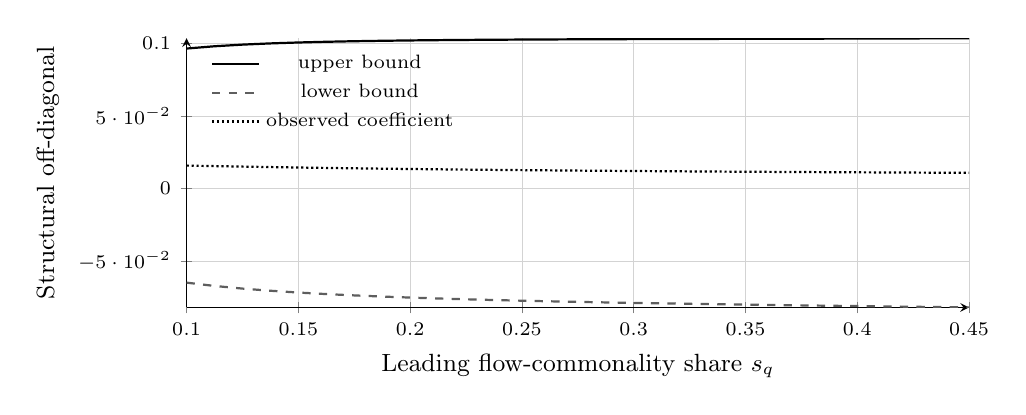
\begin{tikzpicture}
\begin{axis}[
  width=0.95\columnwidth, height=5.0cm,
  xlabel={Leading flow-commonality share $s_q$},
  ylabel={Structural off-diagonal},
  xlabel style={font=\small}, ylabel style={font=\small},
  tick label style={font=\scriptsize},
  legend style={font=\scriptsize,at={(0.02,0.98)},anchor=north west,draw=none,fill=none},
  grid=major, grid style={line width=0.2pt,draw=chartlight!45},
  axis lines=left,
]
\addplot[thick,black] coordinates {\FigBoundsUpper};
\addlegendentry{upper bound}
\addplot[thick,chartgray,dashed] coordinates {\FigBoundsLower};
\addlegendentry{lower bound}
\addplot[thick,densely dotted] coordinates {\FigBoundsObserved};
\addlegendentry{observed coefficient}
\end{axis}
\end{tikzpicture}
\caption{Sharp identified interval for the structural off-diagonal as leading
flow commonality varies, at $s_r=0.32$ and $d=0.29$. The set contains zero
across the whole grid, and the observed coefficient sits far inside it. A
conditional analytic exhibit under the declared one-spike and
isotropic-residual conventions, not a market estimate.}
\label{fig:bounds}
\end{figure}

\subsection{Which functionals survive}
\label{sec:functionals}

Proposition~\ref{prop:sharp} bounds individual entries. The question a user of
the matrix actually faces is different: not \emph{which entries} are pinned
down, but \emph{which numbers computed from the matrix} are. The answer is
clean, and it depends on one thing only.

\begin{theorem}[Identified linear functionals]
\label{thm:linfun}
For $a,b\in\mathbb R^N$ with $a\ne0$, the functional $a^\top\Lambda b$ takes
the same value at every $\Lambda\in\mathcal I(A)$ if and only if
$W^\top b=0$.
\end{theorem}

\begin{proof}
By \eqref{eq:lamAW}, $a^\top\Lambda b=a^\top Ab-(a^\top\Gamma)(W^\top b)$. The
first term is observable; as $\Gamma$ ranges over an open set and $a\ne0$, the
vector $a^\top\Gamma$ ranges over a neighbourhood in $\mathbb R^K$, so the
second term is constant exactly when $W^\top b=0$.
\end{proof}

The condition constrains $b$, the \emph{flow} argument, and says nothing about
$a$. Choosing a response direction orthogonal to the confounding subspace buys
nothing: at our fixture the spread of $a^\top\Lambda b$ across the identified
set is $6.65$ for a free pair and $7.40$ when $a$ is orthogonalised, but
$3.0\times10^{-15}$ when $b$ is.

\begin{theorem}[Identified quadratic costs]
\label{thm:quadfun}
For $x\ne0$, the execution cost $x^\top\Lambda x$ is point identified over
$\mathcal I(A)$ if and only if $W^\top x=0$.
\end{theorem}

Theorem~\ref{thm:quadfun} is Theorem~\ref{thm:linfun} at $a=b=x$; the measured
spread is $13.4$ for a free trade and $3.6\times10^{-15}$ for a
confounding-orthogonal one. It subsumes
Corollary~\ref{cor:pointid}: in the permutation-invariant one-spike geometry
$\Delta_f=h_q m$ and $\Sigma_{qq}m=q_1m$, so $W=(h_q/q_1)m$ and
$\col(W)=\spann(m)$ --- verified to $\lvert\cos\rvert=1.000000000000$. Dollar
neutrality is therefore not a special virtue of dollar-neutral trades. It is
what $W^\top x=0$ happens to reduce to in that one geometry, and it generalises
to no other.

\begin{theorem}[Width of the identified cost interval]
\label{thm:width}
If the admissible loadings satisfy $\lVert\Gamma\rVert_F\le R$, then
\begin{equation}
\operatorname{width}\{x^\top\Lambda x:\Lambda\in\mathcal I(A)\}
=2R\,\lVert x\rVert\,\lVert W^\top x\rVert,
\label{eq:width}
\end{equation}
attained at $\Gamma^\star=R\,xw^\top/\lVert xw^\top\rVert_F$ with $w=W^\top x$.
\end{theorem}

\begin{proof}
$x^\top\Gamma W^\top x=\langle\Gamma,xw^\top\rangle_F$, and the supremum of a
linear functional over a Frobenius ball of radius $R$ is
$R\lVert xw^\top\rVert_F=R\lVert x\rVert\lVert w\rVert$, attained at
$\Gamma^\star$; the infimum is its negative.
\end{proof}

Both the trade's size and its reach into $\col(W)$ enter \eqref{eq:width}, and
the ball is an idealisation of the true positive-semidefiniteness constraint,
so \eqref{eq:width} is an upper bound on the true width, tight when the binding
constraint is spherical.

The economic content of this subsection is a distinction the literature does
not draw. \emph{Parameter identification and decision identification are
different objects.} A desk can hold a completely unidentified impact matrix and
still know exactly what a particular execution will cost, provided that
execution's flow exposure avoids $\col(W)$. Section~\ref{sec:regret} shows the
gap between the two is wider still once the trade is chosen optimally.

\section{A Refutable Restriction}
\label{sec:diagnostic}

Corollary~\ref{cor:set} confines a purely confounded coefficient matrix to
$\mathcal D_K$, which is a proper subset of $\R^{N\times N}$ whenever
$K<N-1$. Membership is therefore refutable.

\begin{definition}[Low-rank departure statistic]
\label{def:psi}
For a coefficient matrix $\widehat A$ and factor count $K$, define
\begin{equation}
\psi_K(\widehat A)
=\frac{\min_{D,\,\rank(R)\le K}\bigl\|\widehat A-D-R\bigr\|_F}
       {\bigl\|\widehat A-\diag(\widehat A)\bigr\|_F},
\label{eq:psi}
\end{equation}
the minimum over diagonal $D$ and rank-$K$ $R$, normalised by total
off-diagonal energy.
\end{definition}

The normalisation makes $\psi_K$ scale-free and invariant to simultaneous
row-and-column permutation of the assets, both verified numerically to
$10^{-12}$.

\begin{proposition}[Population zero]
\label{prop:psizero}
Under $H_0$: $\Lambda$ diagonal, $B=0$, and exactly $K$ latent factors,
$\psi_K(\plim\widehat\Lambda_{\mathrm{OLS}})=0$.
\end{proposition}

\begin{proof}
Immediate from Corollary~\ref{cor:set}: the minimand attains zero at $D=\Lambda$
and $R=G$.
\end{proof}

\paragraph{Direction of the test.} A materially nonzero $\psi_K$ rejects the
maintained pure-confounding null under the stated factor budget. That null
bundles diagonal $\Lambda$, $B=0$, exactly $K$ latent factors, the
zero-cross-covariance restrictions, linearity, and stationarity; rejection
falsifies the conjunction, and genuine structural cross-impact is one
explanation for it rather than the only one. This is the reverse of the conventional reading, under which a
large off-diagonal coefficient is itself the evidence. Under our results
off-diagonal magnitude carries no such information; only departure from
$\mathcal D_K$ does.

\paragraph{Computation and conservatism.} The minimisation in
Eq.~\eqref{eq:psi} is biconvex and is solved by alternating projection: with
$R$ fixed the optimal $D$ is $\diag(\widehat A-R)$, and with $D$ fixed the
optimal $R$ is the rank-$K$ truncated singular value decomposition of
$\widehat A-D$. Each half-step is the exact Frobenius minimiser over its block,
so the objective is nonincreasing and bounded below. The limit is a stationary
point rather than a certified global minimum, so the computed $\psi_K$ is an
\emph{upper bound} on the true distance. That does \emph{not} make the test
conservative: rejection occurs for large values, so an upward-biased statistic
pushes toward more rejection, not less. The optimization error has an a priori
ambiguous effect on rejection probability, and numerical and inferential
validity must therefore be established separately. The alternating projection
itself is standard
\cite{ChandrasekaranEtAl2011}; the contribution here is the economic
restriction it tests.

\paragraph{Two caveats stated up front.} First, $\psi_K=0$ does not prove
$\Lambda$ is diagonal: a structural matrix that is itself
diagonal-plus-rank-$K$ is observationally indistinguishable from a
contaminated diagonal one. The test refutes; it does not confirm. Second,
$\psi_K$ depends on the assumed factor count. Overstating $K$ shrinks the
statistic mechanically and weakens the test; understating it inflates the
statistic and can produce spurious rejection. Any application must report a
sweep over $K$.

Figure~\ref{fig:diagnostic} shows both behaviours. Panel~(a) confirms strict
monotonicity in the size of a genuine structural perturbation. Panel~(b) shows
the factor-count sensitivity, with a pronounced elbow at the true $K=3$: the
statistic falls from $0.6396$ at $K=1$ and $0.3748$ at $K=2$ to $0.0391$ at
$K=3$, then decays slowly. The elbow is a practical way to read the factor
count off the coefficient matrix itself.

\begin{figure}[t]
\centering
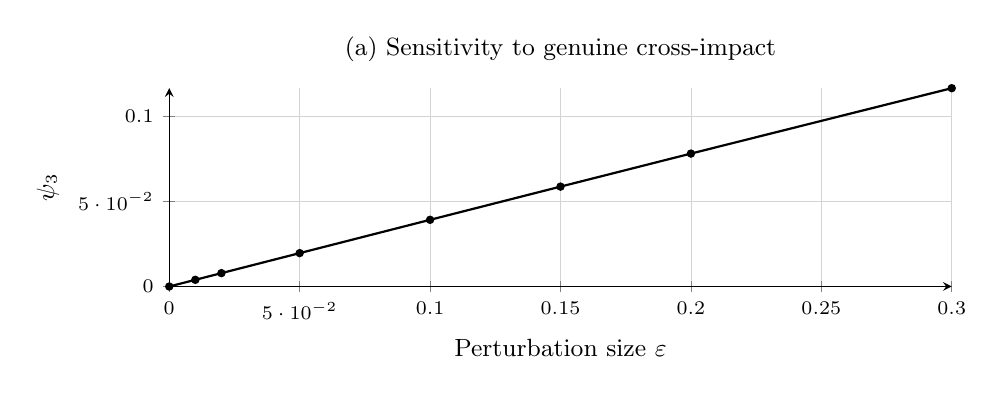
\begin{tikzpicture}
\begin{axis}[
  width=0.95\columnwidth, height=4.1cm,
  title={\small (a) Sensitivity to genuine cross-impact},
  xlabel={Perturbation size $\varepsilon$}, ylabel={$\psi_3$},
  xlabel style={font=\small}, ylabel style={font=\small},
  tick label style={font=\scriptsize},
  grid=major, grid style={line width=0.2pt,draw=chartlight!45},
  axis lines=left,
]
\addplot[thick,black,mark=*,mark size=1.1pt] coordinates {\FigPsiCurve};
\end{axis}
\end{tikzpicture}

\vspace{4pt}

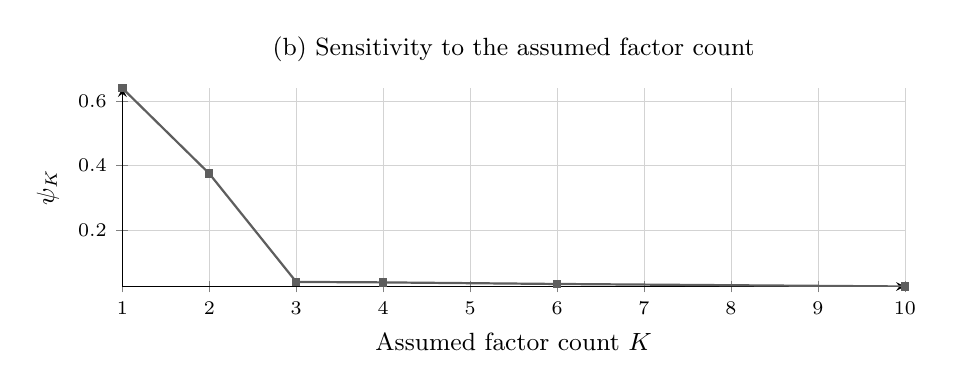
\begin{tikzpicture}
\begin{axis}[
  width=0.95\columnwidth, height=4.1cm,
  title={\small (b) Sensitivity to the assumed factor count},
  xlabel={Assumed factor count $K$}, ylabel={$\psi_K$},
  xlabel style={font=\small}, ylabel style={font=\small},
  tick label style={font=\scriptsize},
  grid=major, grid style={line width=0.2pt,draw=chartlight!45},
  axis lines=left,
]
\addplot[thick,chartgray,mark=square*,mark size=1.1pt] coordinates {\FigPsiByFactorCount};
\end{axis}
\end{tikzpicture}
\caption{The diagnostic under both failure directions. Panel~(a): $\psi_3$ is
zero at exact diagonal-plus-rank-$3$ structure and strictly increasing in a
genuine off-diagonal perturbation. Panel~(b): the statistic is inflated when
the factor count is understated and decays when it is overstated, with an
elbow at the true value $K=3$. Deterministic evaluations at test seed $1729$.}
\label{fig:diagnostic}
\end{figure}

\subsection{Exact restrictions with no nuisance diagonal}
\label{sec:crossblock}

The statistic $\psi_K$ has two defects. It minimises over a diagonal and a
rank-$K$ matrix jointly --- a biconvex, nonconvex problem whose alternating
projection converges to a stationary point that depends on where it started ---
and it must estimate a diagonal nobody wants to know. Both disappear under one
observation.

\begin{theorem}[Cross-block rank]
\label{thm:crossblock}
Let $A=D+R$ with $D$ diagonal and $\rank(R)\le K$, as
Corollary~\ref{cor:set} implies under the maintained null. Then for every pair
of \emph{disjoint} index sets $I\cap J=\varnothing$,
\begin{equation}
A_{I,J}=R_{I,J}\quad\text{and therefore}\quad\rank(A_{I,J})\le K,
\label{eq:crossblock}
\end{equation}
so every $(K+1)\times(K+1)$ minor of $A_{I,J}$ vanishes.
\end{theorem}

\begin{proof}
For $i\in I$ and $j\in J$, disjointness gives $i\ne j$, so
$A_{ij}=D_{ij}+R_{ij}=R_{ij}$. A submatrix cannot exceed the rank of its
parent, and vanishing of all $(K+1)$-minors is the determinantal
characterisation of that bound.
\end{proof}

\begin{corollary}[Tetrads at one factor]
\label{cor:tetrad}
If $K=1$ then $A_{ij}A_{k\ell}-A_{i\ell}A_{kj}=0$ for distinct $i,k\in I$ and
distinct $j,\ell\in J$.
\end{corollary}

These are restrictions on four observed coefficients containing no diagonal and
no unknown parameter of any kind. Testing \eqref{eq:crossblock} needs one
singular value decomposition of an $\lvert I\rvert\times\lvert J\rvert$ block:
no nuisance, no starting point, no convergence criterion. At $N=30$, $K=3$,
with $I=\{0,\dots,9\}$ and $J=\{15,\dots,24\}$, the block reproduces $R_{I,J}$
to machine zero and $\sigma_4(A_{I,J})=4.2\times10^{-17}$; under a dense
off-diagonal perturbation of Frobenius size $\epsilon$ it responds immediately,
reaching $1.27\times10^{-3}$ at $\epsilon=0.01$ and $2.53\times10^{-2}$ at
$\epsilon=0.20$. All $784$ tetrads vanish at $K=1$ (largest
$1.7\times10^{-18}$) and reach $5.9\times10^{-2}$ on a $K=3$ matrix, so the
restriction discriminates the factor count rather than holding vacuously.

\subsection{Is the restriction a characterisation?}
\label{sec:converse}

Theorem~\ref{thm:crossblock} runs one way. Whether its converse holds decides
what a \emph{non}-rejection buys: rejection needs only the forward implication,
but reading non-rejection as evidence \emph{for} pure confounding needs the
other direction. We settle two thirds of the question and are explicit about
the third.

First, when the restriction constrains anything at all. Off-diagonals of
rank-$K$ matrices occupy $K(2N-K)$ dimensions inside the $N^2-N$ dimensional
space of off-diagonal patterns.

\begin{proposition}[Content boundary]
\label{prop:content}
The disjoint cross-block restriction is non-vacuous if and only if
\begin{equation}
K(2N-K)<N^2-N,\qquad\text{equivalently}\qquad K<N-\sqrt N.
\label{eq:content}
\end{equation}
\end{proposition}

\begin{proof}
$K(2N-K)<N(N-1)$ rearranges to $(N-K)^2>N$, and $K<N$ gives $N-K>\sqrt N$.
\end{proof}

Proposition~\ref{prop:content} sits beside Corollary~\ref{cor:empty} as a
second budget constraint. Corollary~\ref{cor:empty} says the \emph{gap} carries
no low-rank structure once $K+\rank(B)\ge N$; \eqref{eq:content} says the
\emph{test} has nothing to detect once $K\ge N-\sqrt N$. At $N=30$ these bind
at $K=30$ and $K=25$, so the registered geometry clears both comfortably.

\begin{theorem}[Global converse at one factor]
\label{thm:converse1}
Let $N\ge4$, let every disjoint tetrad of $A$ vanish, and let the anchors
$A_{01}$, $A_{12}$, $A_{20}$ be nonzero. Then $A_{ij}=x_iy_j$ for all $i\ne j$,
and $D_{ii}=x_iy_i$ gives $\rank(A-D)\le1$.
\end{theorem}

\begin{proof}
Put $x_i=A_{i1}$ for $i\ne1$ and $y_j=A_{0j}/A_{01}$ for $j\ne0$. For $i\ne1$,
$j\ne0$, $i\ne j$ the tetrad on $I=\{i,0\}$, $J=\{j,1\}$ --- disjoint under
exactly those conditions --- gives $A_{ij}A_{01}=A_{i1}A_{0j}$, that is
$A_{ij}=x_iy_j$. The remaining two families follow from a third index, which
exists because $N\ge4$: $x_1=A_{12}/y_2$ and $y_0=A_{20}/x_2$. Replacing the
diagonal of $A$ by that of $xy^\top$ leaves $xy^\top$.
\end{proof}

Reconstructing $x,y$ from off-diagonal entries alone recovers the completion to
$4.4\times10^{-16}$ with $\rank(A-D^\star)=1$ at every $N\in\{4,5,6,8,12\}$. At
$N=3$ no four distinct indices exist, the tetrad family is empty, and the
restriction is silent --- the hypothesis $N\ge4$ is not decorative.

For $K\ge2$ we have no global proof, but the local question is decisive.
Let $S_1$ be the off-diagonals of rank-$K$ matrices and $S_2$ the variety cut
out by all minimal disjoint cross-block $(K+1)$-minors, so
$S_1\subseteq S_2$ by Theorem~\ref{thm:crossblock}. Differentiating the minors
at a generic $D+UV^\top$ gives $\dim T S_2=K(2N-K)=\dim S_1$ in every
configuration we computed, across $K=1,2,3$ and $N=5,\dots,9$.

\begin{corollary}[Local converse]
\label{cor:localconverse}
Near a generic diagonal-plus-rank-$K$ matrix, satisfying every disjoint
cross-block rank bound is equivalent to being completable to rank $K$.
\end{corollary}

We state the residual gap rather than paper over it. Tangent-space equality at
generic points of $S_1$ does not exclude other irreducible components of $S_2$
lying elsewhere, so the following is open: for $K\ge2$, is there an $A$ whose
disjoint cross-blocks all have rank at most $K$ while no diagonal completion
reaches rank $K$? We have neither proved there is none nor found one. The
symmetric analogue is the classical Frisch problem, where non-identified
configurations are known above the Ledermann bound; that governs a different
count --- symmetric covariance rather than an asymmetric coefficient matrix ---
and we do not import it. Practically the gap is narrow: rejection uses only
Theorem~\ref{thm:crossblock}, so refutation is unaffected either way.

\subsection{How much confounding would it take?}
\label{sec:kmin}

Theorem~\ref{thm:crossblock} answers ``given $K$, is the matrix consistent with
pure confounding?'' The more informative question runs the other way. Define
\begin{equation}
K_{\min}(A)=\min_{D\ \text{diagonal}}\rank(A-D),
\label{eq:kmin}
\end{equation}
the smallest latent dimension that could rationalise the observed coefficient
matrix with no structural cross-impact at all. Every disjoint cross-block
certifies a lower bound, since $\rank(A_{I,J})\le K_{\min}(A)$ by
Theorem~\ref{thm:crossblock} applied in reverse.

The decisive empirical comparison is then between $K_{\min}(A)$, read off the
coefficient matrix, and the number of factors $K_{\text{flow}}$ estimated
independently from the order-flow covariance. If
$K_{\min}(A)>K_{\text{flow}}$ with statistical confidence, pure factor
confounding cannot account for the observed cross-impact --- and the statement
is a comparison of two dimensions rather than a single opaque distance.

We report the map $K\mapsto p_K$ over a prespecified range wherever this is
taken to data, and never a chosen factor count. Inference for
$\sigma_{K+1}(\widehat A_{I,J})$ under intraday dependence is a separate
registered design; under sampling that singular value is positive even when the
null holds.

\begin{remark}[A negative result we are obliged to record]
\label{rem:completion}
Recovering the diagonal by alternating projection is \emph{not} reliable.
Started from the observed matrix it recovers $\diag(G)$ to
$4.4\times10^{-16}$; started from twenty random diagonals at scale $5.0$ the
solutions spread by $24.66$, with maximum error $15.37$. The same procedure
fails at $N=5,6,7$ with $K=3$ while succeeding for $N\ge8$, yet a direct test
shows the diagonal is locally identified at those very configurations. Those
failures are algorithmic, not identification failures --- which is precisely
the argument for \eqref{eq:crossblock}, since it needs no completion at all.
\end{remark}

\section{What It Costs to Be Wrong}
\label{sec:cost}

Identification failure is only interesting if it costs something. A desk does
not consume the impact matrix; it consumes the cost of a trade computed through
it. Let a desk execute $x\in\R^N$ and pay expected impact cost
$C(x,M)=x^\top Mx$.

\begin{theorem}[Rank of the cost error]
\label{thm:cost}
For any trade $x$, $C(x,A)-C(x,\Lambda)=x^\top Gx$. Since
$\rank(G)\le K+\rank(B)$ by Theorem \ref{thm:rank}, the error vanishes
identically on a subspace of trade space of dimension at least
$N-K-\rank(B)$.
\end{theorem}

\begin{corollary}[An immune subspace exists, but it has measure zero]
\label{cor:safe}
There exists a linear subspace of trade space, of dimension at least
$N-K-\rank(B)$, on which the cost error vanishes identically. The magnitude of
the spurious off-diagonals does not affect that dimension. \emph{However}, the
set of trades carrying nonzero cost error has full Lebesgue measure whenever
$\mathrm{sym}(G)\neq0$: immunity is a property a desk must construct
deliberately, not one a trade acquires by chance.
\end{corollary}

This is the practical content of the rank bound, and its two halves point in
opposite directions. On one side, a large immune subspace exists: in our
fixture with $N=30$, $K=3$, $B=0$ it has dimension exactly $27$, and a trade
drawn from it has cost error $5.2\times10^{-17}$. On the other, that subspace
is a null set. Drawing $200{,}000$ trades at random from the fixture,
\emph{every one} carried nonzero cost error. A desk is not protected by the
contamination being low rank; it is protected only by deliberately projecting
its trade onto the immune subspace, which requires knowing that subspace.

Two related objects must not be conflated. Since $x^\top Gx=x^\top
\mathrm{sym}(G)x$ with $\mathrm{sym}(G)=(G+G^\top)/2$, the economically
relevant matrix is the symmetric part. Its kernel has dimension at least
$N-2(K+\rank(B))$ --- in the fixture $\rank(\mathrm{sym}(G))=6$ against
$\rank(G)=3$ --- while $\ker(G)$, of dimension at least $N-K-\rank(B)$, is
contained in the immune set for a different reason: $Gx=0$ forces
$x^\top Gx=0$ directly. The exact immune set is neither kernel but the quadric
cone $\{x:x^\top\mathrm{sym}(G)x=0\}$, which is not a subspace.

Which $K$ directions are unsafe depends on the geometry. In a fixture with
generic loadings the equal-weight basket is not special and bears about the
same error as a random trade, $-9.81\%$ against $-9.77\%$. In the
permutation-invariant one-spike geometry, where the confounding direction
\emph{is} the equal-weight direction, Eq.~\eqref{eq:constgap} gives
\begin{equation}
C(x,A)-C(x,\Lambda)=g\,(\mathbf 1^\top x)^2,
\label{eq:exposurelaw}
\end{equation}
so the error is exactly proportional to the squared factor exposure of the
trade. Table \ref{tab:cost} reports the consequence.

\begin{table}[t]
\centering
\caption{Cost error in the one-spike geometry, where the confounding direction
is the equal-weight direction. A conditional analytic exhibit, not a market
estimate.}
\label{tab:cost}
\small
\begin{tabular}{@{}lrrr@{}}
\toprule
Trade & True cost & Error & Relative \\
\midrule
Equal-weight index & 0.4234 & $+0.2296$ & $\mathbf{+54.23\%}$ \\
Random unit vector & 0.2950 & $+0.0160$ & $+5.42\%$ \\
Dollar-neutral pair & 0.2854 & $0$ & $\mathbf{0.00\%}$ \\
\bottomrule
\end{tabular}
\end{table}

An index basket is mispriced by more than half its true cost. A dollar-neutral
pair is mispriced by exactly nothing. The operative question for a practitioner
is therefore not whether the cross-impact matrix is identified, but whether the
trade loads on the confounding direction.

\section{Executing Under Partial Identification}
\label{sec:robust}

Proposition \ref{prop:idset} says the desk cannot learn $\Lambda$. It can still
bound what a trade costs.

\begin{proposition}[Identified cost interval]
\label{prop:costint}
In the one-spike geometry every admissible structural matrix has the form
$\Lambda=A-(t/N)\mathbf 1\mathbf 1^\top$ with $|t|\le T$, so
\begin{equation}
C(x,\Lambda)\in\left[\,C(x,A)-\tfrac{T}{N}(\mathbf 1^\top x)^2,\;
C(x,A)+\tfrac{T}{N}(\mathbf 1^\top x)^2\,\right],
\label{eq:costint}
\end{equation}
and the interval is sharp.
\end{proposition}

The half-width is again governed entirely by factor exposure, which yields the
most useful consequence in the paper:

\begin{corollary}[Cost can be identified where the matrix is not]
\label{cor:pointid}
\emph{In the one-spike geometry}, a dollar-neutral trade has a degenerate cost
interval. Its execution cost is point-identified even though the impact matrix
producing it is set-identified with an interval containing zero.
\end{corollary}

An unidentified parameter does not imply an unidentified cost. The scope
qualifier is essential and easy to lose: dollar-neutrality delivers immunity
only because the one-spike confounding direction \emph{is} the equal-weight
direction. In a general geometry the two come apart. At our fixture with
generic loadings, a trade with $\mathbf 1^\top x=0$ to machine precision still
carries a cost error of $-18.24\%$ of its true cost, because it is not
orthogonal to the confounding subspace. The condition that actually confers
immunity is Theorem \ref{thm:cost}'s, membership of the null space of $G$; the
one-spike geometry merely makes that null space easy to name.

For a desk that must take factor exposure, worst-case cost is
$\widehat C(x)=x^\top A_sx+\tfrac{T}{N}(\mathbf 1^\top x)^2$, convex whenever
$A_s\succeq0$. Minimising it subject to a target $c^\top x=q$ gives

\begin{proposition}[Minimax-cost schedule]
\label{prop:minimax}
$x^*(\pi)=\tfrac12\lambda M(\pi)^{-1}c$ with $M(\pi)=A_s+\pi\mathbf
1\mathbf 1^\top$ and $\lambda=2q/(c^\top M(\pi)^{-1}c)$, evaluated at
$\pi=T/N$. Its factor exposure is weakly smaller than the naive schedule's.
\end{proposition}

\begin{corollary}[When robustness is worthless]
\label{cor:degenerate}
If the constraint pins the factor exposure, $x^*(\pi)=x^*(0)$ for every $\pi$.
This covers a fixed total-quantity constraint $\mathbf 1^\top x=Q$, an
index-like target $c\propto\mathbf 1$, and any target whose unconstrained
optimum is already neutral.
\end{corollary}

Corollary \ref{cor:degenerate} is stated because a desk needs to know when not
to bother. Table \ref{tab:robust} confirms it: robustness earns its keep
precisely when the desk retains discretion over factor exposure, and there it
cuts exposure by roughly eighty percent. The closed form matches a
20{,}000-point grid search over feasible schedules exactly.

\begin{table}[t]
\centering
\caption{Minimax-cost schedule against the naive schedule. Both degenerate
cases were predicted before implementation.}
\label{tab:robust}
\small
\begin{tabular}{@{}lrrr@{}}
\toprule
Target & Improvement & \multicolumn{2}{c}{Exposure $\mathbf 1^\top x$} \\
\cmidrule(l){3-4}
 & & naive & robust \\
\midrule
Index-like, $c=\mathbf 1$ & $0.00\%$ & $+1.000$ & $+1.000$ \\
Neutral, $\mathbf 1^\top c=0$ & $0.00\%$ & $0.000$ & $0.000$ \\
General & $\mathbf{3.11\%}$ & $-0.0663$ & $\mathbf{-0.0130}$ \\
\bottomrule
\end{tabular}
\end{table}

This is a static one-period impact model. It carries no decay kernel, risk
aversion, or timing risk, and supports no profitability claim. The rank
structure of the error does not depend on the schedule, so the immune-subspace
conclusion is expected to survive in a multi-period quadratic-cost model, but
that extension is not proved here.

\subsection{A finite-sample null distribution}
\label{sec:psinull}

Proposition \ref{prop:psizero} is a population statement, which leaves
``materially nonzero'' undefined. We close that gap with a parametric plug-in
bootstrap: refit the null projection $\widehat A_0$ from the estimate, redraw
the estimation error from the ordinary-least-squares sampling law
$\sqrt T(\widehat A_{i\cdot}-A_{i\cdot})\to_d N(0,\sigma_i^2\Sigma_{qq}^{-1})$,
and take the upper $1-\alpha$ quantile of $\psi_K(\widehat A_0+E^*)$ as the
critical value. The factor count is selected by an eigenvalue-ratio rule fixed
before use, so it cannot be chosen after seeing a rejection.

The null manifold has dimension $N+K(2N-K)=201$ against $N^2=900$ free
parameters, so the restriction has codimension $699$. Since $\psi_K(\widehat A)
= O_p(T^{-1/2})$ under $H_0$, the test is consistent against any fixed
alternative outside $\mathcal D_K$.

Table \ref{tab:size} reports a confirmatory study at a seed fixed after the
design was registered. \textbf{The test controls size only for large samples.}

\begin{table}[t]
\centering
\caption{Realised size at nominal $5\%$ and power at $T=5000$, $N=30$, $K=3$,
$B=199$. Monte Carlo standard errors $0.018$ and $0.022$.}
\label{tab:size}
\small
\begin{tabular}{@{}rrrr@{}}
\toprule
$T$ & $T/N^2$ & Plug-in size & Inflated \\
\midrule
500 & 0.56 & 0.267 & 0.000 \\
1{,}000 & 1.11 & 0.127 & 0.000 \\
2{,}000 & 2.22 & 0.100 & 0.000 \\
5{,}000 & 5.56 & \textbf{0.040} & 0.000 \\
\midrule
\multicolumn{4}{@{}l}{\textit{Power at $T=5000$ against perturbation size $\varepsilon$}}\\
\multicolumn{2}{@{}l}{$\varepsilon=0.05$} & \multicolumn{2}{r}{0.070} \\
\multicolumn{2}{@{}l}{$\varepsilon=0.10$} & \multicolumn{2}{r}{0.270} \\
\multicolumn{2}{@{}l}{$\varepsilon=0.20$} & \multicolumn{2}{r}{\textbf{0.870}} \\
\multicolumn{2}{@{}l}{$\varepsilon=0.40$} & \multicolumn{2}{r}{1.000} \\
\bottomrule
\end{tabular}
\end{table}

At $T=5000$, roughly $5N^2$ observations, realised size is $0.040$ against
nominal $0.05$ and power against a Frobenius-$0.20$ alternative is $0.870$.
Below that the test over-rejects badly, reaching $0.267$ at $T=500$. We state
the usable range rather than implying general validity: at $N=30$ the test
should not be used below about $T=5N^2$.

The cause is diagnosed rather than left open. The plug-in null is refitted to
the noisy estimate, so the low-rank fit absorbs part of the estimation error
and the bootstrap statistics are centred too low. We report a failed remedy
alongside the working method: inflating the bootstrap error scale by the
degrees-of-freedom factor $\sqrt{N^2/(N^2-201)}=1.1347$ drives realised size to
exactly zero at every sample size and removes all power, because the bias is in
the centre of the null distribution and not its scale. A centre correction such
as a double bootstrap would require its own design and is not attempted.

\begin{figure}[t]
\centering
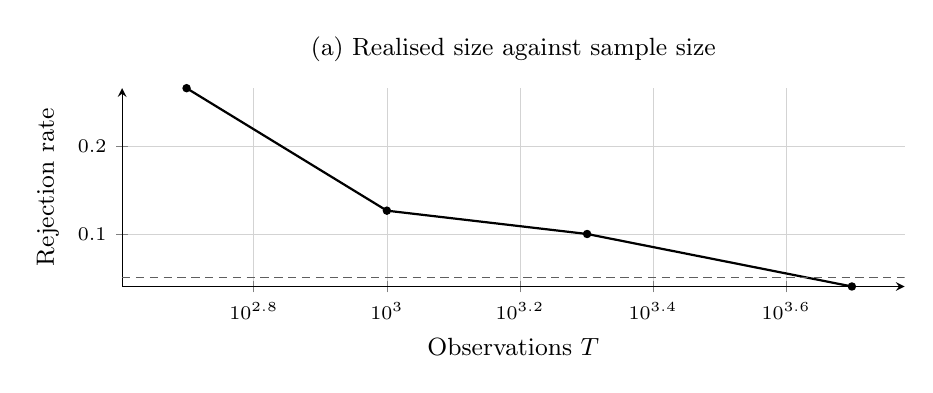
\begin{tikzpicture}
\begin{axis}[
  width=0.95\columnwidth, height=4.1cm,
  title={\small (a) Realised size against sample size},
  xlabel={Observations $T$}, ylabel={Rejection rate},
  xmode=log, log basis x=10,
  xlabel style={font=\small}, ylabel style={font=\small},
  tick label style={font=\scriptsize},
  grid=major, grid style={line width=0.2pt,draw=chartlight!45},
  axis lines=left,
]
\addplot[thick,black,mark=*,mark size=1.1pt] coordinates {\FigPsiSize};
\addplot[densely dashed,chartgray,domain=400:6000,samples=2] {0.05};
\end{axis}
\end{tikzpicture}

\vspace{4pt}

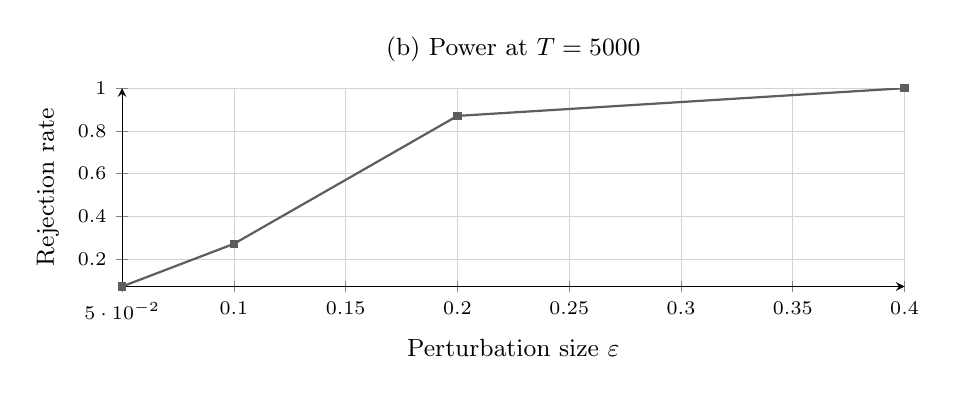
\begin{tikzpicture}
\begin{axis}[
  width=0.95\columnwidth, height=4.1cm,
  title={\small (b) Power at $T=5000$},
  xlabel={Perturbation size $\varepsilon$}, ylabel={Rejection rate},
  xlabel style={font=\small}, ylabel style={font=\small},
  tick label style={font=\scriptsize},
  grid=major, grid style={line width=0.2pt,draw=chartlight!45},
  axis lines=left,
]
\addplot[thick,chartgray,mark=square*,mark size=1.1pt] coordinates {\FigPsiPower};
\end{axis}
\end{tikzpicture}
\caption{The departure test is valid only for large samples. Panel~(a): realised
size against the nominal $5\%$ dashed line; the test over-rejects severely
below roughly $T=5N^2$ and is accurate at $T=5000$. Panel~(b): power against a
dense off-diagonal perturbation at $T=5000$. Monte Carlo standard errors
$0.018$ and $0.022$.}
\label{fig:psistudy}
\end{figure}

\section{What Non-Identification Costs a Trader}
\label{sec:regret}

Sections~\ref{sec:functionals} and \ref{sec:robust} price a \emph{given} trade
under an unidentified matrix. A desk does not trade a given schedule; it
chooses one. The relevant question is what it loses by optimising against the
confounded matrix, and the answer is more forgiving than the identification
results alone suggest.

Let $\Lambda_s=\sym(\Lambda)$ be positive definite --- only the symmetric part
enters, since $x^\top Mx=x^\top\sym(M)x$ --- and let $A_s=\Lambda_s+G_s$ be its
confounded counterpart. A trader completing a position described by one linear
constraint $c^\top x=1$ solves
$x(M)=M^{-1}c/(c^\top M^{-1}c)$ and pays the true cost. Write
\begin{equation}
\mathrm{Regret}=x(A_s)^\top\Lambda_sx(A_s)-x(\Lambda_s)^\top\Lambda_s
x(\Lambda_s).
\label{eq:regretdef}
\end{equation}

\begin{theorem}[Regret is the cost of the trade error]
\label{thm:regret}
With $\delta=x(A_s)-x(\Lambda_s)$,
$\mathrm{Regret}=\delta^\top\Lambda_s\delta\ge0$.
\end{theorem}

\begin{proof}
Both trades satisfy the constraint, so $c^\top\delta=0$. The objective is
quadratic and $x(\Lambda_s)$ minimises it on the affine set, so its gradient
$2\Lambda_sx(\Lambda_s)$ annihilates every feasible direction, giving
$\delta^\top\Lambda_sx(\Lambda_s)=0$. Expanding \eqref{eq:regretdef} and
cancelling the cross term leaves the claim.
\end{proof}

Regret is thus the true cost of the error in the \emph{trade}, never the error
in the matrix. That distinction has teeth.

\begin{theorem}[The damage is second order]
\label{thm:secondorder}
Write $A_s=\Lambda_s+\epsilon G_s$ and set
$\Pi=I-cc^\top\Lambda_s^{-1}/(c^\top\Lambda_s^{-1}c)$. Then
$\delta=-\epsilon\Lambda_s^{-1}\Pi G_sx(\Lambda_s)+O(\epsilon^2)$ and
\begin{equation}
\mathrm{Regret}=\epsilon^2\,(\Pi G_sx_L)^\top\Lambda_s^{-1}(\Pi G_sx_L)
+O(\epsilon^3),\qquad x_L=x(\Lambda_s).
\label{eq:secondorder}
\end{equation}
\end{theorem}

\begin{proof}
The first-order condition is $A_sx=\mu c$ with $c^\top x=1$. Perturbing,
$\Lambda_s\delta+\epsilon G_sx_L=(\mathrm d\mu)c+O(\epsilon^2)$, so
$\delta=\Lambda_s^{-1}((\mathrm d\mu)c-\epsilon G_sx_L)$; imposing
$c^\top\delta=0$ fixes $\mathrm d\mu$ and yields the stated form. Substituting
into Theorem~\ref{thm:regret} gives \eqref{eq:secondorder}.
\end{proof}

\emph{A first-order error in the impact matrix produces only a second-order
loss in execution.} At $N=20$ with $\lVert G_s\rVert_F=1$, halving $\epsilon$
divides the regret by $3.91$, $3.95$, $3.98$ --- approaching the factor of four
\eqref{eq:secondorder} requires --- and the ratio
$\mathrm{Regret}/\epsilon^2$ rises monotonically to the predicted
$0.003388738$. At $\epsilon=0.4$ the trader forgoes $0.87\%$ of optimal cost;
at $\epsilon=0.05$, $0.015\%$. Theorem~\ref{thm:regret} holds to
$1.1\times10^{-17}$ across the grid.

\begin{corollary}[Gaps the trader never feels]
\label{cor:freegap}
$\mathrm{Regret}=0$ if and only if $\Pi G_sx_L=0$, that is
$G_sx_L\in\spann(c)$. In particular any $G_s\propto\Lambda_s$ costs nothing,
the argmin being scale invariant.
\end{corollary}

This is the decision-side counterpart of Theorem~\ref{thm:quadfun}. There, a
trade whose flow exposure avoids $\col(W)$ has a point-identified cost. Here, a
confounding gap that moves the optimal trade only along the constraint
direction costs nothing at all, whatever it does to the matrix entries.

We claim no more than the setting allows: one linear constraint, positive
definite $\Lambda_s$, static and frictionless, no risk term and no alpha, and a
\emph{local} second-order statement whose constant may be large --- at
$\epsilon=0.4$ the observed ratio already departs from its limit by $4\%$.
Identification is not restored. The trader still cannot learn $\Lambda$; the
result says only that this particular decision is insensitive to what cannot
be learned.

\section{Restoring Identification}
\label{sec:restore}

Everything so far is negative or partial: what cannot be learned, what survives
anyway, what a failure of the null would refute. A useful identification paper
should also say what \emph{would} suffice. Here it takes exactly one more
observable.

Fix $B=0$ and the model $r=\Lambda q+\Gamma f+u$, $q=\Delta f+v$. Suppose we
observe two noisy measurements of the same latent factor,
\begin{equation}
h^{(1)}=f+\varepsilon_1,\qquad h^{(2)}=f+\varepsilon_2,
\label{eq:proxies}
\end{equation}
with $\varepsilon_1,\varepsilon_2$ mean zero, uncorrelated with each other and
with $f$, $u$, and $v$. Neither proxy alone identifies $\Lambda$: by
Remark~\ref{rem:control}, controlling for one noisy proxy merely relocates the
estimate within the identified set. Two do.

\begin{theorem}[Two-proxy identification]
\label{thm:twoproxy}
Under \eqref{eq:proxies}, if $\Sigma_f$ is nonsingular and
$\Sigma_{vv}=\Sigma_{qq}-\Delta\Sigma_f\Delta^\top$ is nonsingular, then
\begin{align}
\Sigma_f&=\operatorname{Cov}(h^{(1)},h^{(2)}), \label{eq:sigf}\\
\Delta&=\operatorname{Cov}(q,h^{(1)})\,\Sigma_f^{-1}, \label{eq:delta}\\
\Lambda&=\bigl[\Sigma_{rq}-\Sigma_{rh}\Delta^\top\bigr]
\bigl[\Sigma_{qq}-\Delta\Sigma_f\Delta^\top\bigr]^{-1},
\label{eq:twoproxy}
\end{align}
with $\Sigma_{rh}=\operatorname{Cov}(r,h^{(1)})$. All three right-hand sides
are functions of observable second moments, so $\Lambda$ is point identified.
\end{theorem}

\begin{proof}
Independence of the measurement errors gives
$\operatorname{Cov}(h^{(1)},h^{(2)})=\Sigma_f$, which is \eqref{eq:sigf}. Then
$\operatorname{Cov}(q,h^{(1)})=\operatorname{Cov}(\Delta f+v,f)=\Delta\Sigma_f$
yields \eqref{eq:delta}. Since $\varepsilon_1$ is uncorrelated with $r$'s
disturbances, $\Sigma_{rh}=\operatorname{Cov}(r,f)=\Lambda\Delta\Sigma_f
+\Gamma\Sigma_f$, while
$\Sigma_{rq}=\Lambda\Sigma_{qq}+\Gamma\Sigma_f\Delta^\top$. Substituting
$\Gamma\Sigma_f=\Sigma_{rh}-\Lambda\Delta\Sigma_f$ into the second and
collecting terms gives
$\Sigma_{rq}-\Sigma_{rh}\Delta^\top=\Lambda(\Sigma_{qq}
-\Delta\Sigma_f\Delta^\top)$, which inverts to \eqref{eq:twoproxy}.
\end{proof}

The economic reading is direct. \emph{One noisy proxy for the common factor
does not identify structural cross-impact; two conditionally independent
proxies do.} The second proxy is not extra precision --- it is the instrument
that separates the factor from its measurement error, and with the factor
separated the confounding channel $\Gamma$ drops out of \eqref{eq:twoproxy}
entirely.

Two invertibility conditions carry real content rather than technical
convenience. If $\Sigma_f$ is singular, some factor has no variance and its
loading is unidentified. If $\Sigma_{vv}$ is singular, order flow is driven
purely by the common factors, there is no idiosyncratic flow variation left to
trace impact with, and no amount of proxy quality repairs it. Our
implementation refuses both, judging the second against the scale of
$\Sigma_{qq}$ rather than against the residual's own scale, since a numerically
zero residual has full rank relative to itself.

What Theorem~\ref{thm:twoproxy} does not do is tell an empiricist where to find
two conditionally independent proxies. Candidates --- order flow from disjoint
venues, non-overlapping trader cohorts, alternating time slices --- all
plausibly share microstructure noise, and the conditional independence in
\eqref{eq:proxies} is an assumption on that noise, not a consequence of
disjointness. It is testable in the overidentified case $K<\dim h$, and we
regard establishing it in real data as the substantive empirical hurdle rather
than a formality.

\section{Known-Truth Verification}
\label{sec:verify}

The probability limits were frozen before simulation code and random-number
access, then evaluated along two algebraically independent population paths and
tested in a single registered draw with $N=30$, $K=3$, and
$T=10{,}000{,}000$ independent Gaussian observations. The fixture is
deliberately nontrivial, with $\rho(B\Lambda)=0.4104$ and flow-covariance
condition number approximately $348.1$.

The gate statistic was the maximum elementwise relative discrepancy across both
coefficient matrices, with no denominator floor, element exclusion, averaging
substitute, or seed retry; passage required $D_{\mathrm{gate}}<10^{-3}$.

\begin{table}[t]
\centering
\caption{Completed known-truth verification and the new deterministic checks.}
\label{tab:g1}
\small
\begin{tabular}{@{}p{0.56\columnwidth}>{\raggedleft\arraybackslash}p{0.35\columnwidth}@{}}
\toprule
Quantity & Verified value \\
\midrule
\multicolumn{2}{@{}l}{\textit{Registered $T=10^7$ experiment}}\\
Assets / factors / observations & $30/3/10^7$ \\
Reported coefficients & 1,800 \\
OLS max relative discrepancy & $5.6395\times10^{-4}$ \\
Proxy-control max discrepancy & $5.1237\times10^{-4}$ \\
Gate threshold & $1.0\times10^{-3}$ \\
Targets inside intervals & 1,800 / 1,800 \\
\midrule
\multicolumn{2}{@{}l}{\textit{Rank bound, $\rank(G)$ observed vs.\ $K+\rank(B)$}}\\
$\rank(B)=0$ & 3 vs.\ 3 \\
$\rank(B)=1$ & 4 vs.\ 4 \\
$\rank(B)=2$ & 5 vs.\ 5 \\
$\rank(B)=30$ & 30 vs.\ 33 \\
\midrule
\multicolumn{2}{@{}l}{\textit{Diagnostic}}\\
$\psi_3$ at exact structure & $0$, below a $10^{-12}$ floor \\
Permutation-invariance residual & $<10^{-12}$ \\
One-spike gap constancy & $<10^{-12}$ \\
Closed form vs.\ bisection & $<10^{-10}$ \\
\bottomrule
\end{tabular}
\end{table}

Table~\ref{tab:g1} reports the outcome. The sole frozen draw passed, and all
1,800 target coefficients lay inside named 95\% family-wise classical
homoskedastic Student-$t$ Bonferroni intervals. Immediate replay reused all
validated checkpoints and reproduced the summary, estimates, and success marker
byte for byte.

The lower panels report the new checks. The rank bound binds exactly at every
arm where it can bind and is never violated; at $\rank(B)=30$ the observed rank
is capped by the asset count. The diagnostic attains its predicted population
zero and both invariances. Every entry in these two panels is a deterministic
algebraic evaluation at test seed $1729$, so no interval method applies and no
stochastic comparison is performed.

What this establishes is narrow. The symbolic expressions and the primitive
covariance implementation agree; row-stacked software returns the expected
transpose; and the streamed sufficient-statistic path recovers the registered
target at the intended dimension. It does not establish identification,
empirical fit, causal timing, interval coverage under market dependence, or
economic usefulness.

\section{Confronting Published Evidence}
\label{sec:published}

Equation~\eqref{eq:constgap} yields a prediction that can be checked against
already-published summary statistics without touching market data. In the
permutation-invariant geometry a single factor control shifts \emph{every}
cross-coefficient by one common constant. Two implications follow, and they can
disagree.

\paragraph{Dispersion should be invariant.} A constant shift moves the
cross-sectional mean and leaves the cross-sectional standard deviation
unchanged. Capponi and Cont \cite{CapponiCont2020} report a mean cross
coefficient moving from $0.032$ to $-0.039$, a shift of $-0.071$, while the
cross-sectional standard deviation stays at $0.06$; the own-coefficient
standard deviation moves only from $0.78$ to $0.77$. Both changes are at or
within the reported two-decimal precision. This is the predicted signature, and
it is unit-free, so it requires none of the variable standard deviations the
source does not report.

\paragraph{Distribution shape should be invariant too, and here the check
fails.} Under an exactly constant shift the post-control negative fraction
should equal the pre-control mass lying below the shift magnitude. A Gaussian
approximation to the reported mean and standard deviation puts that at
$0.7422$, against a reported $0.8446$ -- a gap of $0.1024$, exceeding our
declared tolerance of $0.05$.

We report the failure rather than remove it. The registered protocol forbids
retuning the one-spike convention to close such a gap. The most likely
explanation is loading heterogeneity beyond one common factor, which the
one-spike convention assumes away and which the Gaussian approximation to an
empirically skewed cross-section compounds. Note also that the discrepancy does
not bear on Theorem~\ref{thm:rank}, which is an inequality in $K$ and is not
weakened by the presence of additional factors; it bears on the sharper
constant-shift specialisation of Eq.~\eqref{eq:constgap}.

Both checks are conditional analytic exhibits at published summary statistics.
Neither is an estimate of any market's impact matrix, and the published
dispersion figures are not confidence intervals and are not treated as such.

\section{Registered Falsification Protocol}
\label{sec:premise}

The empirical stage is governed by a protocol registered before any data is
opened. Its question is deliberately narrower than identification:

\begin{quote}
Can confounding alone be materially large in a transparent model whose
observable flow commonality and factor alignment match opened primary-source
summaries, even when the estimator receives a favourable factor proxy?
\end{quote}

The design sets $B=0$, so a positive result cannot be explained by price
chasing. It retains $N=30$, uses one permutation-invariant factor, sets proxy
reliability to $0.95$, and evaluates 17 frozen homogeneous structural
off-diagonal values from $0.0029$ to $0.0046$. Three smooth estimators bind at
every grid point: an observable integrated-top-ten-OFI proxy-control
condition-ridge estimator, an oracle-flow condition-ridge estimator, and an
oracle-flow homogeneous three-slope OLS. The first is the binding observable
opponent; the two oracles remove measurement error and high-dimensional
inversion as alternative explanations.

A reconstruction of six published specifications supplies a separate veto.
Because the source paper does not disclose feature scaling, fold chronology,
penalty grid, tie rule, or solver tolerance, the executable version is a
preregistered protocol reconstruction rather than author code, and every
omitted numerical choice is frozen in advance.

For focal estimate $\widehat\Lambda_{01}$, truth $o$, and a standard error from
499 shared whole-date bootstrap replicates, passage requires
\begin{equation}
\bigl|\widehat\Lambda_{01}-o\bigr|-0.50|o|>3\,SE_{\mathrm{boot}}.
\label{eq:gate}
\end{equation}
Before the research draw can exist, 100 independent validation superpanels must
license the exact final procedure through a null-grid size condition and a
power condition with named Clopper--Pearson and Wilson bounds.

The interpretation of every branch is fixed in advance. If all binding
candidates pass, the result supports material confounding within the registered
source-matched model class only. If any binding candidate fails, the protocol
does not pass, and no diagnostic can rescue it. If size, power, numerical,
provenance, or resource admission fails, the research draw stays sealed as a
design failure rather than a market null. A premise-killing null requires a
separately registered sharp upper bound over the source-compatible class; a
single negative fixture is insufficient.

\textbf{This protocol is specified here, not reported.} No registered
stochastic stream has run.

\section{Limitations}

The completed evidence is narrow by construction. The known-truth fixture is
Gaussian and large-sample, its zero contemporaneous shock cross-covariances are
substantive assumptions, and its dense positive targets do not reproduce the
small, sign-sensitive coefficients central to the empirical debate. Interval
inclusion there is one realisation, not an estimated coverage probability.

The new results carry their own limits. Theorem~\ref{thm:rank} is an
inequality, so a high observed rank is uninformative if $K$ is misspecified,
and the rank of the gap is not separately observable from the rank of a
genuinely low-rank $\Lambda$. Proposition~\ref{prop:idset} assumes $B=0$; with
feedback the identified set is larger, not smaller, so
Corollary~\ref{cor:sign} is conservative in that direction only. The closed
form of Proposition~\ref{prop:sharp} is conditional on the one-spike and
isotropic-residual conventions, which are declared maximum-entropy choices and
not identified features of any exchange. The $\psi_K$ statistic is an upper
bound from a stationary point, has no derived sampling distribution here, and
cannot confirm diagonality.

The published-evidence exercise of Section~\ref{sec:published} uses summary
statistics that carry no inferential intervals, so it supports consistency
statements only and admits no $p$-value.

Finally, predictive performance and structural identification remain distinct.
An estimator can forecast well while targeting the wrong impact matrix, and a
structurally interpretable estimator can be economically useless after costs.
Nothing here supports a trading rule, execution-cost saving, or deployment
claim.

\section{Conclusion}

Off-diagonal return-on-flow coefficients do not identify structural
cross-impact by notation alone, and the failure has a precise shape. The gap
between the population coefficient and the structural matrix has rank at most
$K+\rank(B)$. That single fact carries the paper: it explains why a diagonal
truth can generate a dense cross-impact matrix of realistic magnitude, why the
structural matrix is set-identified rather than point-identified, why a factor
control moves an estimate along the contamination rather than out of it, and
why the resulting ambiguity is wide enough at published commonality levels to
leave the structural off-diagonal unsigned.

The same fact supplies the remedy. Low rank is refutable, and $\psi_K$
measures departure from it with the polarity the problem requires: rejection is
evidence for genuine cross-impact, not against it. Whether real markets reject
is an empirical question this paper deliberately does not answer. It registers
the protocol that will, and reports the theory that makes the answer
interpretable when it arrives.

\section*{Declarations}

{\small
\noindent\textbf{Authorship.} Mehmet Demir G\"uven is the sole author. He
conceived the research question, fixed the design and the preregistered
constraints under which it was carried out, directed the work, reviewed and
accepted the results reported here, and takes full responsibility for the
content of this paper, including any errors it contains.

\smallskip
\noindent\textbf{Computational assistance.} Generative AI tools were used
during this project to assist with algebraic derivation, software
implementation, and manuscript preparation. Every formal result was checked
against independent numerical verification, every reported value regenerates
from committed deterministic code, and the preregistration, derivations, and
decision ledgers are public so that any claim can be traced to the evidence
behind it. Responsibility for the correctness of the work rests with the
author. No AI system is an author of this paper.

\smallskip
\noindent\textbf{Funding and institutional status.} This independent research
received no funding from ETH Z\"urich. The affiliation records the author's
status as a computer science student only. ETH Z\"urich did not sponsor,
approve, or endorse the research, and the paper does not represent the
university's views.

\smallskip
\noindent\textbf{Data and code availability.} No external market data was
accessed. Every numerical value reported here is regenerated by committed,
deterministic code with a single command; the repository, preregistration,
derivations, and ledgers are public.

\smallskip
\noindent\textbf{Competing interests.} The author declares none.

\smallskip
\noindent\textbf{License.} Copyright \textcopyright\ 2026 Mehmet Demir
G\"uven. This preprint, its source, and its figures are licensed under
\href{https://creativecommons.org/licenses/by/4.0/}{CC BY 4.0}. This license
applies to the article, not automatically to repository software,
configurations, data, or result artifacts.
}

\appendix

\section{Proof of Theorem \ref{thm:plim}}
\label{app:plim}

From Eqs.~\eqref{eq:return}--\eqref{eq:flow},
$(I-B\Lambda)q_t=(B\Gamma+\Delta_f)f_t+Bu_t+v_t$, which yields
Eq.~\eqref{eq:q-reduced}. Mutual zero cross-covariances give
$\Cov(f_t,q_t)=\Sigma_fP^\top$ and $\Cov(u_t,q_t)=\Sigma_uU^\top$. Using
$r_t=\Lambda q_t+\Gamma f_t+u_t$,
\begin{equation}
\Sigma_{rq}=\Lambda\Sigma_{qq}+\Gamma\Sigma_fP^\top+\Sigma_uU^\top,
\end{equation}
and right multiplication by $\Sigma_{qq}^{-1}$ proves
Eq.~\eqref{eq:ols-plim}.

For the proxy-controlled regression, the linear-projection residual of $f_t$
after controlling for $h_t=f_t+\epsilon_t$ is
$f_t^\perp=f_t-\Sigma_f(\Sigma_f+\Sigma_\epsilon)^{-1}h_t$ with variance
$R_f$. Frisch--Waugh--Lovell residualisation gives
$q_t^\perp=Pf_t^\perp+Uu_t+Vv_t$ and
$r_t^\perp=\Lambda q_t^\perp+\Gamma f_t^\perp+u_t$, so $\Var(q_t^\perp)=Q_h$
and $\Cov(r_t^\perp,q_t^\perp)=\Lambda Q_h+\Gamma R_fP^\top+\Sigma_uU^\top$.
Right multiplication by $Q_h^{-1}$ proves Eq.~\eqref{eq:proxy-plim}.
\hfill$\square$

\section{Proof of Proposition \ref{prop:idset}}
\label{app:idset}

\emph{Necessity.} Any structural tuple consistent with the observables must
satisfy Eq.~\eqref{eq:lamAW} by Theorem~\ref{thm:rank} with $B=0$, and its
residual covariances must be positive semidefinite.

\emph{Sufficiency.} Given $(\Gamma,\Delta_f)$ satisfying both semidefiniteness
constraints, set $\Lambda=A-\Gamma W^\top$, $\Sigma_v=\Sigma_{qq}-\Delta_f
\Delta_f^\top$, and $\Sigma_u$ as stated. The resulting tuple is a valid
instance of Eqs.~\eqref{eq:return}--\eqref{eq:flow} with $B=0$, and reversing
the algebra reproduces $\Sigma_{qq}$, $\Sigma_{rr}$, and $\Sigma_{rq}$.
Hence every element of $\mathcal I$ is observationally equivalent.
\hfill$\square$

\section{Proof of Proposition \ref{prop:sharp}}
\label{app:sharp}

Decompose every matrix in the $m$ direction and its orthogonal complement, on
which all matrices act as multiples of the identity.

First, $\Sigma_v=\Sigma_{qq}-\Delta_f\Delta_f^\top=q_0I\succeq0$
automatically, imposing no restriction.

Next, $\Lambda m=\lambda_1m$ with $\lambda_1=d+(N-1)o$, and $\Lambda$ acts as
$(d-o)I$ on $m^\perp$. With $\Gamma=\gamma m$ and $\Cov(q_t,f_t)=h_qm$,
\begin{equation}
\Sigma_u=\Sigma_{rr}-\Lambda\Sigma_{qq}\Lambda^\top
-(2\gamma h_q\lambda_1+\gamma^2)mm^\top.
\end{equation}
On $m^\perp$ the eigenvalue is $r_0-(d-o)^2q_0$; since $d-o=A_{\mathrm{diag}}
-A_{\mathrm{off}}$, this is free of $t$ and restricts nothing. On $m$ the
eigenvalue is $r_1-\lambda_1^2q_1-2\gamma h_q\lambda_1-\gamma^2$, so
$\Sigma_u\succeq0$ requires
\begin{equation}
\gamma^2+2\lambda_1h_q\gamma+\lambda_1^2q_1-r_1\le0.
\end{equation}
Substituting $\gamma=tq_1/h_q$ and $\lambda_1=a_1-t$, the middle terms combine
as $q_1(a_1-t)(a_1+t)=q_1(a_1^2-t^2)$, giving
\begin{equation}
\frac{t^2q_1^2}{q_1-q_0}+q_1a_1^2-q_1t^2\le r_1,
\end{equation}
that is $t^2q_1q_0/(q_1-q_0)\le r_1-q_1a_1^2$, which is Eq.~\eqref{eq:T}.
Since $\Lambda_{\mathrm{off}}=A_{\mathrm{off}}-t/N$, Eq.~\eqref{eq:sharp}
follows.
\hfill$\square$

\section{Proof of Theorem \ref{thm:generic}}
\label{app:generic}

Write $b=\rank(B)$. The matrix $M^\top\Sigma_{qq}^{-1}$ is invertible, so the
second block of $R$ in \eqref{eq:gapfactor}, namely
$B_L^\top M^\top\Sigma_{qq}^{-1}$, has full row rank $b$. Positive definiteness
of $\Sigma_f$ together with $\rank(P)=\rank(M(B\Gamma+\Delta_f))=K$ makes
$\Sigma_fP^\top\Sigma_{qq}^{-1}$ of full row rank $K$. Under
\eqref{eq:nooverlap} the two blocks have independent row spaces, since a
nontrivial relation among them would exhibit a nonzero vector of the
intersection; hence $\rank(R)=K+b$.

For $L$: $\rank(\Gamma)=K$ by hypothesis, and $\Sigma_{uu}B_R^\top$ has rank
$b$ because $\Sigma_{uu}$ is invertible and $B_R$ has full row rank.
Condition~\eqref{eq:nooverlap} says their column spaces meet only at the
origin, so $\rank(L)=K+b$.

Both factors therefore have rank $K+b$, and the inner dimension of the product
is exactly $K+b$. Sylvester's rank inequality gives
$\rank(LR)\ge\rank(L)+\rank(R)-(K+b)=K+b$, while \eqref{eq:gapfactor} bounds
$\rank(LR)\le K+b$. \qed

\section{Equivalent Primitive Forms}

With $\Omega_q=D\Sigma_fD^\top+B\Sigma_uB^\top+\Sigma_v$ and
$\Omega_{q\mid h}=DR_fD^\top+B\Sigma_uB^\top+\Sigma_v$, and using
$\Sigma_{qq}=H\Omega_qH^\top$ and $Q_h=H\Omega_{q\mid h}H^\top$,
Theorem~\ref{thm:plim} is equivalently
\begin{align}
\plim\widehat\Lambda_{\mathrm{OLS}}
&=\Lambda+(\Gamma\Sigma_fD^\top+\Sigma_uB^\top)\Omega_q^{-1}(I-B\Lambda), \\
\plim\widehat\Lambda_{q\mid h}
&=\Lambda+(\Gamma R_fD^\top+\Sigma_uB^\top)\Omega_{q\mid h}^{-1}(I-B\Lambda).
\end{align}
These forms show the decomposition is determined entirely by structural
primitives under the stated zero-cross-covariance assumptions, and make the
rank bound of Theorem~\ref{thm:rank} visible directly in the primitives.

\begingroup
\small
\setlength{\itemsep}{1pt plus 0.2pt minus 0.2pt}
\bibliographystyle{plain}
\bibliography{references}
\endgroup

\end{document}
